%
% Chapter 12
%

\chapter{RESULTS}
\label{chap:results}
The main purpose of this analysis is to measurment the best-fit signal strength parameter $\mu = \sigma/\sigma_{SM}$ of the \tth signal process.
This is done by comparing the observed number of events in data to the expected number of events from background plus \tth signal with a Higgs boson of mass 125 GeV. 
This signal strength $\mu$ is the factor by which the expected \tth yields are multiplied, without altering the branching fractions, to best-fit the observation in data
while the backgrounds are constrained to SM predictions within their systematic uncertainties. We also report 95$\%$ CL upper limits on $\mu$ for the SM \tth process.

\section{Upper Limits}
The 95$\%$ upper limits on $\mu$ are obtained with the $CL_{s}$ method using the asymptotic approximation of the profile likelihood, described in Section~\ref{sec:limit}.
The observed (median expected under background-only hypothesis) upper limit on $\mu$ is 2.9 (1.0$^{+0.5}_{-0.3}$), as shown in Table~\ref{tab:limits}.

\begin{table}[htbp]
\begin{center}
  \caption[Table of Final Limits]{95$\%$ CL upper limits on $\mu$ under the background-only hypothesis.}
    \begin{tabular}{c c} \hline
      Observed Limit & Expected Limit $\pm$1$\sigma$  \\ \hline 
      2.9 & 1.0$^{+0.5}_{-0.3}$  \\
      \hline
    \end{tabular}
    \label{tab:limits}
\end{center}
\end{table}

\section{Signal Strength}
The signal strength parameter best fit $\mu$ was obtained with the Maximum Likelihood Estimator method described in Section~\ref{sec:fit}.
The observed (expected) best fit signal strength for the SM \tth hypothesis is 1.7$^{+0.6}_{-0.5}$ (1.0$^{+0.5}_{-0.5}$) times the SM expectation,
corresponding to an observed (expected) significance of 3.3$\sigma$ (2.1$\sigma$), as shown in Table~\ref{tab:mu}.
The post-fit yields for the expected signal and background processes are listed by lepton flavor in Table~\ref{tab:postfit_yields}.
The impacts of the statistical, theoretical, and experimental sources of uncertainty, as well as the post-fit values of the nuisances and their correlation with
the fitted signal strength is shown in Figure~\ref{fig:impacts}.

\begin{table}[htbp]
\begin{center}
  \caption[Table of best-fit signal strength]{}
    \begin{tabular}{c c c} \hline
      Observed $\mu$ fit $\pm$1$\sigma$ & Expected $\mu$ fit $\pm$1$\sigma$ & Observed(expected) significance & \\ \hline 
      1.7$^{+0.6}_{-0.5}$ & 1.0$^{+0.5}_{-0.5}$ & 3.3$\sigma$ (2.1$\sigma$)  \\
      \hline
    \end{tabular}
    \label{tab:mu}
\end{center}
\end{table}


\begin{table}[htbp]
  \begin{center}
    \caption[Signal region post-fit event yields by lepton flavor]{Expected (post-fit) yields for signal and background processes, and observed yields in data. Yields
      shown after a fit to data with all predictions constrained to SM expectation.}
    \begin{tabular}{l c c c} \hline
      & $\mu\mu$ & $ee$ & $e\mu$  \\ \hline 
      $t\bar{t}W$ & 51.2 $\pm$ 2.6 & 20.4 $\pm$ 1.0 & 72.9 $\pm$ 3.4 \\
      $t\bar{t}Z/\gamma^{*}$ & 17.9 $\pm$ 0.9 & 16.0 $\pm$ 1.0 & 44.9 $\pm$ 2.0 \\
      \hline
      WZ & 6.8 $\pm$ 2.6 & 2.0 $\pm$ 0.8 & 10.0 $\pm$ 3.5 \\
      Rare SM. bkg & 7.2 $\pm$ 0.8 & 4.0 $\pm$ 0.4 & 12.5 $\pm$ 1.1 \\
      WWss & 3.6 $\pm$ 0.7 & 1.8 $\pm$ 0.3 & 5.5 $\pm$ 1.0 \\
      \hline
      Conversions & 0.0 $\pm$ 0.0 & 10.7 $\pm$ 6.3 & 7.4 $\pm$ 1.2 \\
      Charge flip & 0.0 $\pm$ 0.0 & 9.2 $\pm$ 0.8 & 14.2 $\pm$ 1.2 \\
      Non-prompt leptons & 31.9 $\pm$ 5.8 & 18.4 $\pm$ 2.4 & 56.7 $\pm$ 7.3 \\
      \hline
      Total bkg & 118.6 $\pm$ 7.0 & 82.6 $\pm$ 7.0 & 224.1 $\pm$ 9.3 \\
      \hline
      $t\bar{t}H$ & 19.5 $\pm$ 1.4 & 7.9 $\pm$ 0.6 & 27.6 $\pm$ 1.9 \\
      \hline
      Data & 154 & 95 & 274 \\
      \hline
    \end{tabular}
    \label{tab:postfit_yields}
  \end{center}
\end{table}


\begin{figure}[htb]
        \centering 
        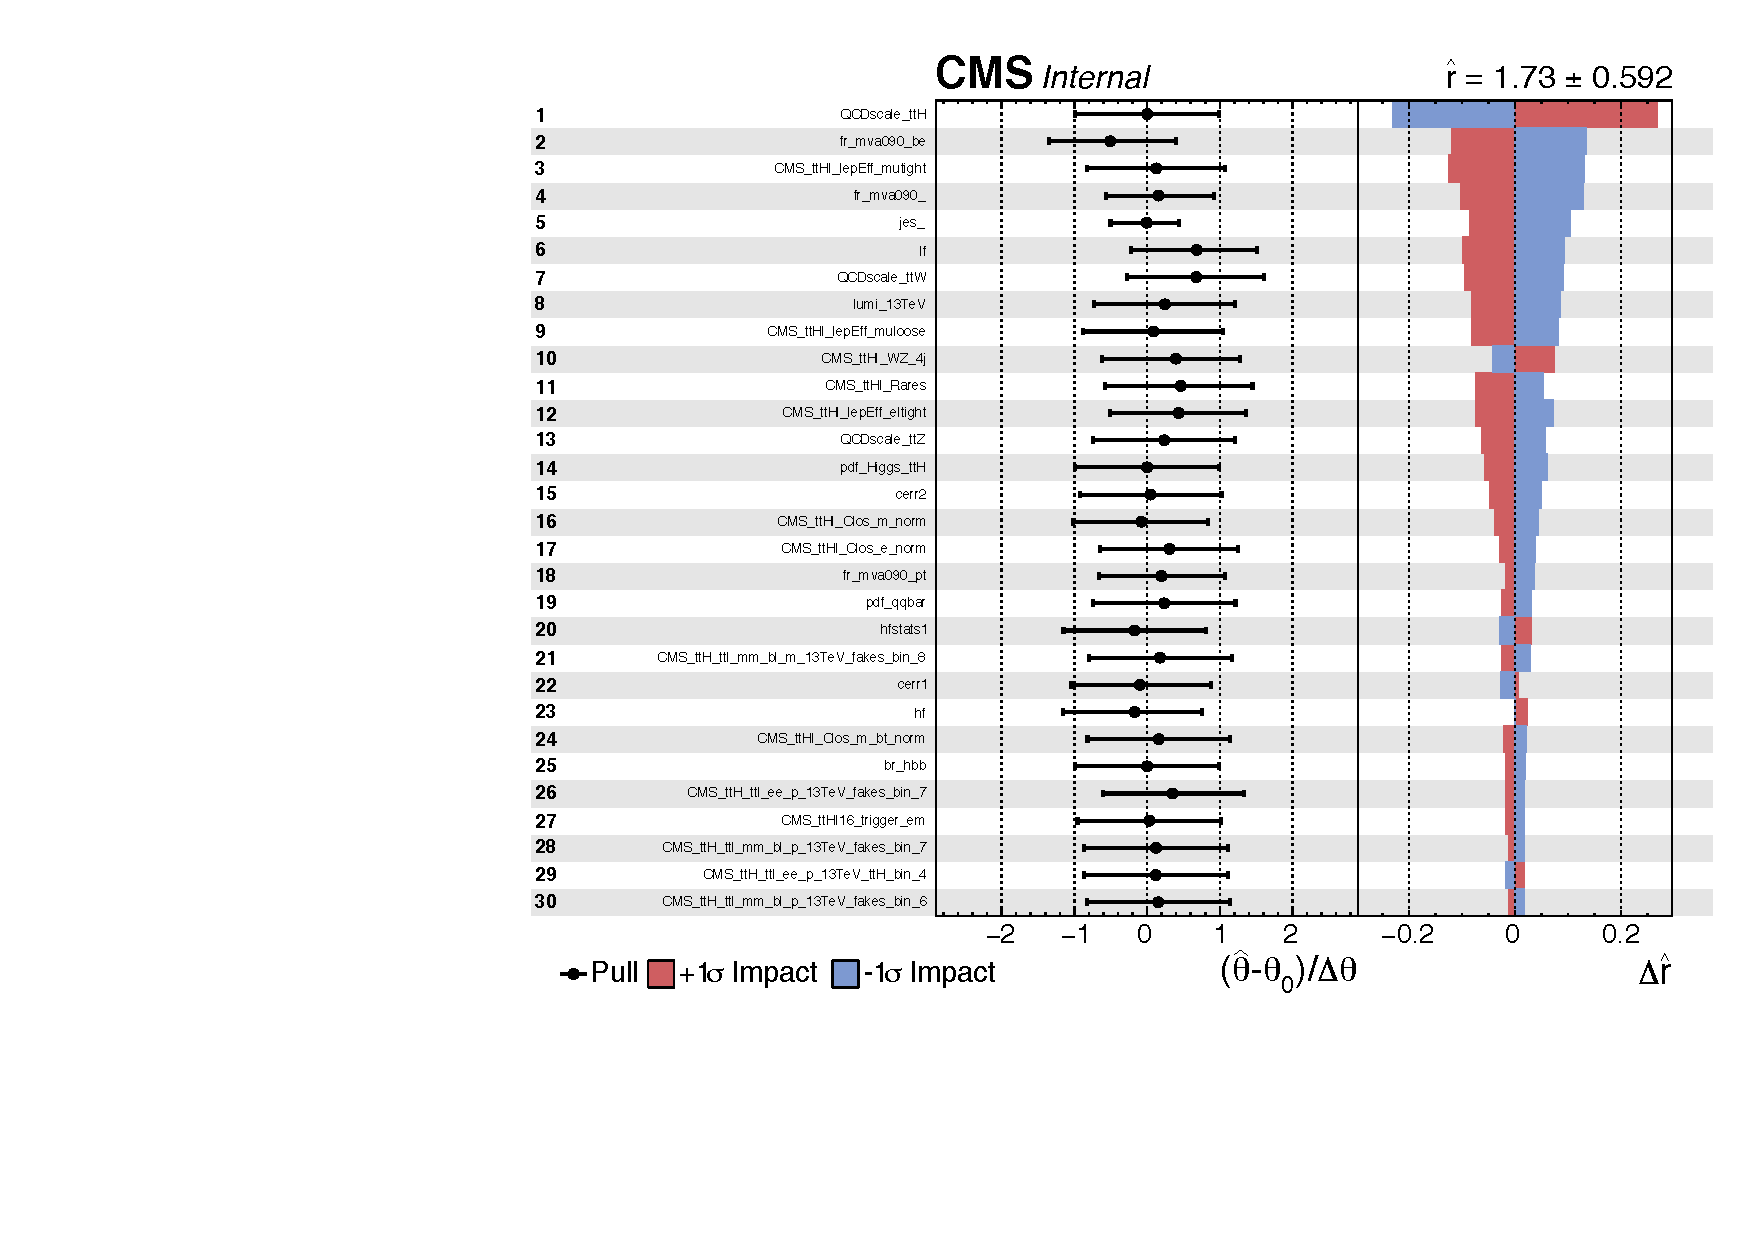
\includegraphics[width=0.95\textwidth]{ch11_figs/impacts_ttH_13TeV_top30.pdf}
        \caption[Nuisance parameter impacts]{The top nuisance parameters ranked by their impact on the fit. The pull of each nuisance (left) is the amount by which the fit moves that parameter from its
        initial value. The impact of each nuisance (right) is the change in best-fit $\mu$ divided by the uncertainty in $\mu$, obtained by moving each nuisance up (red) or down (blue) by 1$\sigma$.}
        \label{fig:impacts}
\end{figure}



\section{Conclusion}
This dissertation presents a complete measurement of the \tth signal strength, targeting the $WW*$, $ZZ*$, and $\tau\tau~*$ decays of the Higgs boson
in the two same-sign leptons channel at $\sqrt{s} = 13$ TeV with an integrated luminosity of 35.9$fb^{-1}$.
The data analyzed corresponds to the full dataset collected by the CMS experiment in 2016.
This analysis presented represents the most precise measurement of \tth in the $2lss$ channel to-date.
The signal and background are estimated with MC, with the exception of the backgrounds due to fake leptons and charge mis-assignments,
which are estimated with data. A BDT discriminant is constructed using kinematic and reconstruction-based BDT scores as input variables.
This discriminant is binned and used to extract the signal via a maximum likelihood fit in each of the ten sub-categories of the signal region.
This analysis is the first of its kind to observe evidence for SM \tth above the 3$\sigma$ significance level and represents significant
improvements over previous iterations, thanks in part, to increased separation power provided by reconstruction BDTs that target the hadronic top
and the jets from the Higgs. This analysis directly probes the SM via the top-Higgs Yukawa coupling, and while a small excess is observed
in the $e\mu$ and $\mu\mu$ channels, the observation is consistent with the SM within 1$\sigma$. 

In addition to testing the SM, this analysis demonstrates the performance improvement offered from reconstruction-oriented BDTs. With the inclusion of the BDTs
which reconstruct the Higgs jets and the hadronic top portions of the \tth event as inputs to the final BDTs,
the discrimination power improves by nearly 10$\%$ from the ROC curves. These reconstruction-oriented techniques show promising results and could be useful
in other analyses with complicated final states.

Finally, the work presented here is included in a publication scheduled to appear in the journal Physical Review B. 
